\documentclass{report}
\usepackage[utf8]{inputenc}
\usepackage[letterpaper,top=3cm,bottom=3cm,left=3cm,right=3cm,marginparwidth=1.75cm]{geometry}
\usepackage{indentfirst}
\usepackage{graphicx}
\usepackage{geometry}
\usepackage{lmodern}

\renewcommand*\contentsname{Sommaire}
\renewcommand{\listfigurename}{Table des figures}
\renewcommand{\chaptername}{Chapitre}

\begin{document}
\begin{center}
République Algérienne Démocratique et Populaire\\
Ministre de l'Enseignement Supérieur et de la Recherche Scientifique\\
Université Abderrahmane Mira - Béjaïa\\
\rule{0.75\textwidth}{1 pt}\\

\includegraphics[scale=0.7]{logo.jpg}\\
\rule{0.75\textwidth}{1pt}\\[0.25 cm]
Faculté des Sciences Exactes\\
Département Informatique\\
\rule{0.75\textwidth}{1pt}\\[0.5 cm]
\LARGE Projet fin de cycle\\
\rule{0.95\textwidth}{2 pt}\\
\Large Thème\\
\Large Conception et réalisation d’une application mobile de livraison de produits alimentaires\\
\rule{0.95\textwidth}{2 pt}\\[1 cm]
Rédigé par:\\[0.5 cm]
\begin{tabular}{lll}
\hline\hline\\
ZAIDI & Melissa & C4\\
YOUSFI & Souhila & C4\\
YOUS & Sabrina & C4\\
TETAH & Ikram & C4\\
TITOUN & Rami & C4\\
TOUATI & Yanis & C4\\
ZIDOUNI & Nacereddine & C4\\[1 cm]
\end{tabular}\\
Encadré par : AIT ABDELOUAHAB Karima\\[1 cm]
Année Universitaire: 2021-2022
\end{center}
\thispagestyle{empty}
\newpage

\clearpage
\pagenumbering{arabic}

\tableofcontents
\newpage

\chapter{Contexte du travail et méthodologie du développement.}

\section{Introduction}
De nos jours, plusieurs supérettes rencontrent des difficultés de gestion de stock et des livraisons en suivant les méthodes classiques, ce qui peut provoquer des pertes d’informations, de temps et d'argent.

En plus du manque de fiabilité des méthodes obsolètes, la crise du Covid-19 a gelé l'économie mondiale pendant des mois, il a fallu alors se pencher sur des méthodes plus modernes et efficaces.

Par conséquent nous allons, à travers ce projet, mettre en place une application mobile complète qui automatisera la gestion des supérettes et de ses livraisons, tout en veillant à ce qu’elle soit rapide, efficace et simple d’utilisation.

Dans ce chapitre, nous mettrons l’accent sur l’analyse préliminaire du projet, c'est-à-dire définir le domaine du projet ainsi que les problématiques liées à celui-ci et les solutions pouvant être apportées.

\section{Présentation du projet}
Ce projet se présente sous la forme d'une application mobile Java qui aura pour but de faciliter la gestion des supérettes, de leur stock, et la satisfaction de leur clientèle.

Cette application offrira une expérience semblable à un vrai magasin dans le sens où le choix ne sera pas limité et la méthode de paiement sera d'autant plus facile. Pour acheter des produits de ces magasins virtuels, il suffira simplement de sélectionner les produits souhaités et de les ajouter au panier.

L’acheteur peut alors remplir le bon de commande et payer la commande par carte de crédit ou autre moyen de paiement. Les commandes seront affectées à un livreur qui se chargera de livrer le panier à l'acheteur de manière automatisée et optimale.

\subsection{Étude de l’existant}
Pour acheter des produits alimentaires comme les fruits, les légumes, la viande, etc. Les clients doivent se rendre directement à un magasin pour trouver une offre de vente répondant à leurs besoins. Cette procédure peut être inutile et même être une perte de temps, de plus, même le vendeur n’aura aucun moyen de publier ses annonces de ventes ou de services sauf dans les médias traditionnels tels que les journaux et les petites affiches. Le personnel du magasin adopte également les méthodes traditionnelles :

\begin{itemize}
    \item Le règlement des factures en espèce ou par chèque, sur place.
    \item L’enregistrement des clients manuellement sur papier.
    \item La vérification de la disponibilité des produits et leur validité.
    \item La gestion minutieuse du stock.
    \item Calcul du montant total.
\end{itemize}

Vu l’accroissement de la technologie Internet, l’achat en ligne (l'e-commerce) est devenu une nécessité incontournable pour les commerçants pour faciliter la vente et diminuer les risques d'erreurs humaines à travers l'automatisation des tâches. Ainsi, cette application que nous réaliserons sera un moyen fiable d’informer un grand nombre de clients d'offres commerciales et des services nécessaires.

\subsection{Commerce traditionnel et e-commerce}
L'e-commerce fait pression sur les magasins de proximité à travers ses divers avantages en garantissant :

\begin{itemize}
    \item La disponibilité des produits et leur visibilité : Un site de vente en ligne est disponible 24 h/24 et 7 jours/7, il est donc visible à tout moment. Les horaires ne pénalisent donc pas plus les vendeurs des produits ou des services. Ainsi tous les consommateurs ayant des horaires décalés seront toujours ciblés. En bref, les clients peuvent commander d'où ils veulent et quand ils veulent.
    \item Des coûts moins élévés : à travers la simplicité des modes de paiement, l'acheteur peut commander et payer plus facilement. Le vendeur peut ainsi en faire profiter sa clientèle, en proposant des prix plus bas que dans une boutique physique. La rapidité du e-commerce permet le choix, la sélection des articles, et le paiement en quelques clics tandis qu’en magasin le client peut subir une longue file d’attente ou même négocier avec le vendeur.
    \item Un nombre d’utilisateurs important : La VPC (vente par correspondance) simplifie tout le processus d’achat et attire donc un plus grand nombre d'utilisateurs. De ce fait, le secteur du e-commerce vit un essor depuis quelques années, en témoigne le dernier rapport de la FEVAD (Fédération du e-commerce et de la vente à distance) de 2021 <<En 2021, les ventes en ligne ont progressé de 15,1\%. Le secteur du e-commerce (Produits et Services) a dépassé les 129 milliards d'euros en 2021, en hausse de 15,1\%, contre 8,5\% en 2020. Le secteur retrouve ainsi une croissance à deux chiffres.>>
\end{itemize}

D’autre part pour assurer une bonne réputation de la marque, il est essentiel que la marque soit présenté sur internet. En effet, les commentaires en ligne disponibles au public sur internet mènent à accroître ou à décroître la réputation de la marque, le commerce en ligne n’est pas toujours rentable.

L'e-commerce gagne encore un point en offrant l'option de livraison rapide et automatisée par la géo-localisation comme il est pour objet d'étude de notre projet.

\section{Problématique et objectifs du travail}
Après avoir fait l’étude de l’organisme d’accueil, nous allons analyser les problèmes rencontrés par les membres du personnel d’une supérette ou par le client puis nous tenterons d’apporter des solutions.

\subsection{Problématique}
La gestion des supérette se fait manuellement, ce qui engendre plusieurs problèmes tels que :

\begin{itemize}
    \item Des erreurs de calcul engendrées par la gestion manuelle.
    \item Utilisation de plusieurs documents (facture, bon de livraison, liste des produits livrés), ce qui entraîne une mauvaise organisation de ces derniers.
    \item Une perte de temps pour le client parce qu’il doit se déplacer à la supérette pour acheter ce qu’il veut.
    \item Perte de dossiers, bons de livraisons, factures ce qui nous oblige à les refaire donc un coût financier supplémentaire et une perte de temps considérable.
    \item La gestion des livraisons se fait manuellement ce qui peut occasionner l’oubli ou le chevauchement des livraisons.
    \item Manque d’informations sur les produits et donc se fier à la mémoire humaine ce qui peut en résulter un effet catastrophique sur le système au complet.
    \item Environnement de travail stressant pour le ou les employés, causé par toute cette masse de données à prendre en considération lors de n’importe quelle livraison.
    \item Absence de vérification de la disponibilité des produits.
\end{itemize}

C’est dû à ces contraintes citées en haut que nous avons réfléchi à établir un plan de conception d’une application de livraison des produits alimentaires qui permettra de faciliter les achats tout en répondant aux besoins des utilisateurs.

\subsection{Objectifs du travail}
Notre projet consiste à réaliser une application mobile qui permettra la livraison des produits alimentaires de supérettes. La conception et le développement de notre application vise à atteindre les objectifs suivants :

\begin{itemize}
    \item Multiplier la force de vente.
    \item Gérer les livraisons.
    \item Gagner du temps par rapport au client, il peut acheter ce qu’il veut sans besoin de sortir de chez lui.
    \item Donner plus d’informations sur les produits alimentaires : date limite de consommation, prix...
    \item Assurer une livraison rapide du produit et dans un état parfait.
    \item Stockage d’informations dans une base de données afin de minimiser leurs pertes.
    \item Sécuriser l’accès aux informations par une authentification.
    \item Faciliter la recherche et l’accès aux informations ainsi que leurs mises à jour.
    \item Informer les clients sur les promotions faites.
    \item En cas d’endommage ou d’expiration du produit le client a le droit de le signaler.
    \item Permettre au client de donner son avis.
\end{itemize}

\section{Quelques définitions concernant le projet}

\subsection{Définition d'une application mobile}
Une application mobile est un logiciel applicatif développé pour un appareil électronique mobile, tel qu'un assistant personnel, un téléphone portable, un smartphone, ou une tablette tactile.

Environ 200 milliards d'applications mobiles ont été téléchargées jusqu'en 2015, alors qu'en 2009, deux milliards seulement l'avaient été. En 2017, 178,1 milliards d'applications mobiles ont été téléchargées. En 2018, le chiffre se monte à 205,4 milliards selon l'étude Statista dans <<Annual number of mobile app downloads worldwide 2022 Statistic>>.

\subsection{Définition du commerce}
Le commerce désigne l'activité économique d'achat et de revente de biens et de services, en particulier l'achat dans le but de revendre avec un profit ou un bénéfice. Le commerce a ses lois propres qui sont recueillies dans les Code de commerce et ses propres juridictions nationales ou internationales.

Dans le cas de la vente des produits alimentaires, il s'agit de la vente de tout article fabriqué ou présenté comme pouvant servir de nourriture ou de boisson à l'être humain.

\subsection{Définition de l'e-commerce}
Le E-commerce ou <<commerce électronique>> est l’utilisation d’un média électronique pour la réalisation de transactions commerciales. Il s’agit généralement de la vente de produits à travers le réseau Internet, mais le terme de E-commerce correspond également aux mécanismes d’achat par Internet.

Au début des années 1990, Phil Brande Berger a passé la première commande en ligne en utilisant un système de paiement sécurisé par carte de crédit, Le New York Times couvre l’évènement et souligne que <<derrière un petit clic pour un individu se cache un grand pas pour l’économie mondiale>>.

\subsection{Méthode de paiement en ligne}
Le contrat électronique en ligne passe par le paiement des services et des biens. Le paiement est l’aspect le plus controversé du commerce électronique car il demeure l’obstacle à son développement face au risque encore assez important de fraude et de piratage.

En effet seules les méthodes sur le paiement sur le réseau pourront favoriser la confiance des opérateurs : banques, commerçants, utilisateurs ... Pourtant, les risques de détournement d’un numéro de carte bancaire sur le réseau ne sont pas plus grands que ceux l’empreinte laissée après un paiement. La recherche de moyens de paiement plus surs assurera sans doute le développement du commerce électronique notamment par la cryptographie.

\section{Méthode de développement utilisée}
La méthode de développement utilisée dans ce projet est la méthode du processus
unifié (PU) traduit de l’anglais unified process (UP). Ce processus de développement a été choisi car il est moderne, efficace et complet. Il est aussi adapté à une large classe de systèmes logiciels, à différents domaines d'application et à différents types et tailles d'entreprises.

\subsection{Définition du processus unifié (PU)}
Le processus unifié est un processus de développement logiciel itératif et incrémental centré sur l'architecture et les modèles UML. Il est piloté par les cas d’utilisation et orienté vers la diminution des risques avec pour but de regrouper les activités à mener pour transformer les besoins d'un utilisateur en système logiciel.

\subsection{L'architecture bidirectionnelle du processus unifié}
Le processus unifié gère le processus de développement par deux axes :

L'axe vertical : représente les principaux enchaînements d'activités, qui regroupent les activités selon leur nature. Cette dimension rend compte l'aspect statique du processus qui s'exprime en terme de composants, de processus, d'activités, d'enchaînements, d'artefacts et de travailleurs.

L'axe horizontal : représente le temps et montre le déroulement du cycle de vie du processus; cette dimension rend compte de l'aspect dynamique du processus qui s'exprime en terme de cycles, de phases et d'itérations.

\begin{figure}[!htb]
\centering
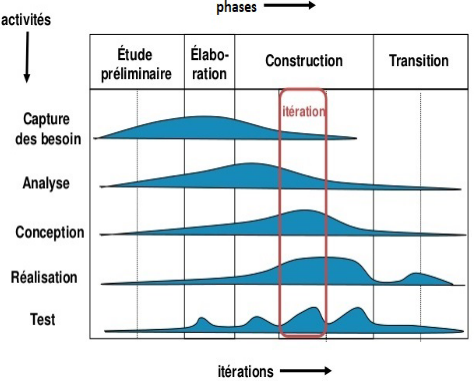
\includegraphics[width=9 cm]{processus UP.png}
\begin{center}
\caption{Schéma du processus unifié par Y.Prié, <<Processus de conception de SI>>, Département d'informatique, Université Claude Bernard Lyon 1, (2011-2012).}
\end{center}
\end{figure}

\subsection{Les activités}
\subsubsection{Expression des besoins}
Elle permet de définir les différents besoins qui sont :

\begin{itemize}
    \item Inventorier les besoins principaux et fournir une liste de leurs fonctions
    \item Recenser les besoins fonctionnels (du point de vue de l'utilisateur) qui conduisent à l'élaboration des modèles de cas d'utilisation.
    \item Appréhender les besoins non fonctionnels (techniques) et livrer une liste des exigences.
\end{itemize}

\subsubsection{Analyse}
L'objectif de l'analyse est d'accéder à une compréhension des besoins et des exigences du client. Il s'agit de livrer des spécifications pour permettre de choisir la conception de la solution. Un modèle d'analyse livre une spécification complète des besoins issus des cas d'utilisation et les structures sous une forme qui facilite la compréhension (scénarios), la préparation (définition de l'architecture), la modification et la maintenance du futur système.

\subsubsection{Conception}
La conception permet d'acquérir une compréhension approfondie des contraintes liées au langage de programmation, à l'utilisation des composants et au système d'exploitation. Elle détermine les principales interfaces et les transcrit à l'aide d'une notation commune.

\subsubsection{Implémentation}
L'implémentation est le résultat de la conception pour implémenter le système sous forme de composants, c'est-à-dire, de code source, de scripts, de binaires, d'exécutables et d'autres éléments du même type.

Les objectifs principaux de l'implémentation sont de planifier les intégrations des composants pour chaque itération, et de produire les classes et les sous-systèmes sous forme de codes sources.

\subsubsection{Tests}
Les tests permettent de vérifier des résultats de l'implémentation en testant la construction. Il faut les planifier pour chaque itération, les implémenter en créant des cas de tests, effectuer ces tests et prendre en compte le résultat de chacun.

\subsection{Les phases}
\subsubsection{Analyse des besoins}
L'analyse des besoins donne une vue du projet sous forme de produit fini. Cette phase porte essentiellement sur les besoins principaux (du point de vue de l'utilisateur), l'architecture générale du système, les risques majeurs, les délais et les coûts

\subsubsection{Élaboration}
L'élaboration reprend les éléments de la phase d'analyse des besoins et les précise pour arriver à une spécification détaillée de la solution à mettre en œuvre. Elle permet de préciser la plupart des cas d'utilisation, de concevoir l'architecture du système et surtout de déterminer l'architecture de référence.


Au terme de cette phase, les chefs de projet doivent être en mesure de prévoir les activités et d'estimer les ressources nécessaires à l'achèvement du projet.

\subsubsection{Construction}
La construction est le moment où l'on construit le produit. L'architecture de référence se métamorphose en produit complet. Le produit contient tous les cas d'utilisation que les chefs de projet en accord avec les utilisateurs ont décidé de mettre au point pour cette version.

\subsubsection{Transition}
Le produit est en version bêta. Un groupe d'utilisateurs essaie le produit et détecte les anomalies et défauts. Cette phase suppose des activités comme la formation des utilisateurs clients, la mise en œuvre d'un service d'assistance et la correction des anomalies constatées.

\section{Conclusion}
L’étude de l’existant permet donc de comprendre et d’analyser les différentes activités d'un organisme dans le but de dégager des critiques et de ce fait proposer des solutions. Les applications informatiques sont conçues dans le but de concrétiser ces solutions pour améliorer les services des organismes.

Et donc, la réalisation d’une application informatique nécessite une étude conceptuelle détaillée à travers la capture des besoins de cette dernière qui sera l’objet d'étude du chapitre suivant.

\chapter{Analyse et spécification des besoins}

\end{document}
 